\section{Realisierung}
\label{sec:realisierung}

Das Simulationstool ist eine Modifikation einer Software, die als \enquote{Traffic Simulation Game} für einen Workshop für Doktoranden\footnote{https://lightjason.github.io/news/2017-09-workshop/} erstellt wurde.

In diesem Workshop mussten die Teilnehmer mit Hilfe der Agentensprache ein Fahrzeug so steuern, dass dieses auf einem 50 km langen Straßenstück, welches zufällig Bereiche mit Geschwindigkeitsbegrenzungen enthielt, möglichst wenige Strafzettel erhielten.

Für die Zwecke dieser Arbeit musste die Software angepasst werden.
Dabei mussten während der Tests der ersten Agentenpläne Korrekturen vorgenommen werden, da sonst eine fehlerfreie Simulation nicht möglich gewesen wäre. 
Mehr dazu nachfolgend in \cref{sec:anpassungen-probleme}.





\subsection{Anpassungen der Simulationssoftware}
\label{sec:anpassungen-probleme}

Einer der Hauptunterschiede zur Softwareversion des Workshops ist, dass die Simulationen hier auf einer unendlichen Strecke stattfinden.
Fahrzeuge, die das Streckenende passieren, werden mit gleichen Verhaltenswerten am Anfang wieder eingesetzt.
Dieses Umsetzen selbst bereitete keine Probleme, allerdings resultierten solche aus der Unterbrechung der Strecke.



\subsubsection{Schwierigkeiten bei der Simulation der Ringform der Strecke}
\label{sec:probleme-ringform}

Die Streckenunterbrechung führte dazu, dass es eine Pause in der Sichtbarkeit der Fahrzeuge untereinander gab, wenn sich diese an unterschiedlichen Enden der Strecke befanden.
Aufgrund dieser \enquote{Unsichtbarkeit} ergab sich die Unmöglichkeit der Berechnung zwischen den einzelnen Fahrzeugen und führte zu einer freien Beschleunigung, da eine freie Strecke vermutet wurde.

Nachfolgend ist dies anhand eines Auszugs aus einem Log einer Simulation mit zwei Fahrzeugen dargestellt.
\enquote{...} bezeichnet Kürzungen der Ausgabe.

In Zeitschritt 315 war Fahrzeug vehicle20 gerade noch in der letzten Zelle der Fahrbahn und überschreitet diese Grenze einen Zeitschritt später.
Die Beliefliste beider Fahrzeuge ist ab dem Schritt 316 leer.
Erst nach vier Zeitschritten befindet sich auch das Folgefahrzeug (vehicle0) am Anfang der Fahrspur und ist ab Zeitschritt 320 wieder für Fahrzeug 20 sichtbar (andersherum ebenso).

\footnotesize\begin{verbatim}
----- step 315 ----------------
      vehicle0   -> BELIEFLIST   [view/vehicle[id[vehicle20], ... direction[forward[]]]]]]
      vehicle20   -> BELIEFLIST   [view/vehicle[id[vehicle0], ... direction[backward[]]]]]]
      vehicle0   in lane   1   in cell   331.0   @   87.11188616490347   kph
      vehicle20   in lane   1   in cell   400.0   @   88.65039571533352   kph
----- step 316 ----------------
      vehicle0   -> BELIEFLIST   []
      vehicle20   -> BELIEFLIST   []
      vehicle0   in lane   1   in cell   345.0   @   87.89778423377561   kph
      vehicle20   in lane   1   in cell   14.0   @   88.65039571533352   kph
----- step 317 ----------------
...
----- step 318 ----------------
...
----- step 319 ----------------
      vehicle0   -> BELIEFLIST   []
      vehicle20   -> BELIEFLIST   []
      vehicle0   in lane   1   in cell   387.0   @   89.01152857206483   kph
      vehicle20   in lane   1   in cell   56.0   @   88.65039571533352   kph
----- step 320 ----------------
      vehicle0   -> BELIEFLIST   [view/vehicle[id[vehicle20], ... direction[forward[]]]]]]
      vehicle20   -> BELIEFLIST   [view/vehicle[id[vehicle0], ... direction[backward[]]]]]]
      vehicle0   in lane   1   in cell   1.0   @   89.79742664093698   kph
      vehicle20   in lane 1 in cell 70.0 @ 88.65039571533352 kph
\end{verbatim}
\normalsize

Für die Simulation mit mehreren Fahrzeugen stellte dies insbesondere ein Problem dar, weil eine Stauwelle, die sich in ihrer Rückwärtsbewegung dem Anfang der Strecke näherte, von Fahrzeugen am Ende der Strecke nicht erkannt werden konnte.
Dies führte zu dem Verhalten, dass Fahrzeuge vom Ende der Strecke an den Anfang gesetzt werden sollten, dort aber nicht in eine freie Zelle gesetzt werden konnten.
Die Simulationsumgebung sieht hier vor, dass das Fahrzeug auf die freie Zelle hinter das jeweils letzte Fahrzeug gesetzt wird - also im negativen Bereich.
Allerdings wurden die Fahrzeuge, die sich bereits dort befanden, jeweils noch ein Feld weiter nach hinten gesetzt und das neue Fahrzeug dazwischen einfügt.

Es ergab sich bei Simulationsläufen ein Häufung von Positionspunkten im negativen Teil der Strecke, siehe \cref{figure:negativ-sammeln}.
\begin{figure}[hptb]
 \centering
 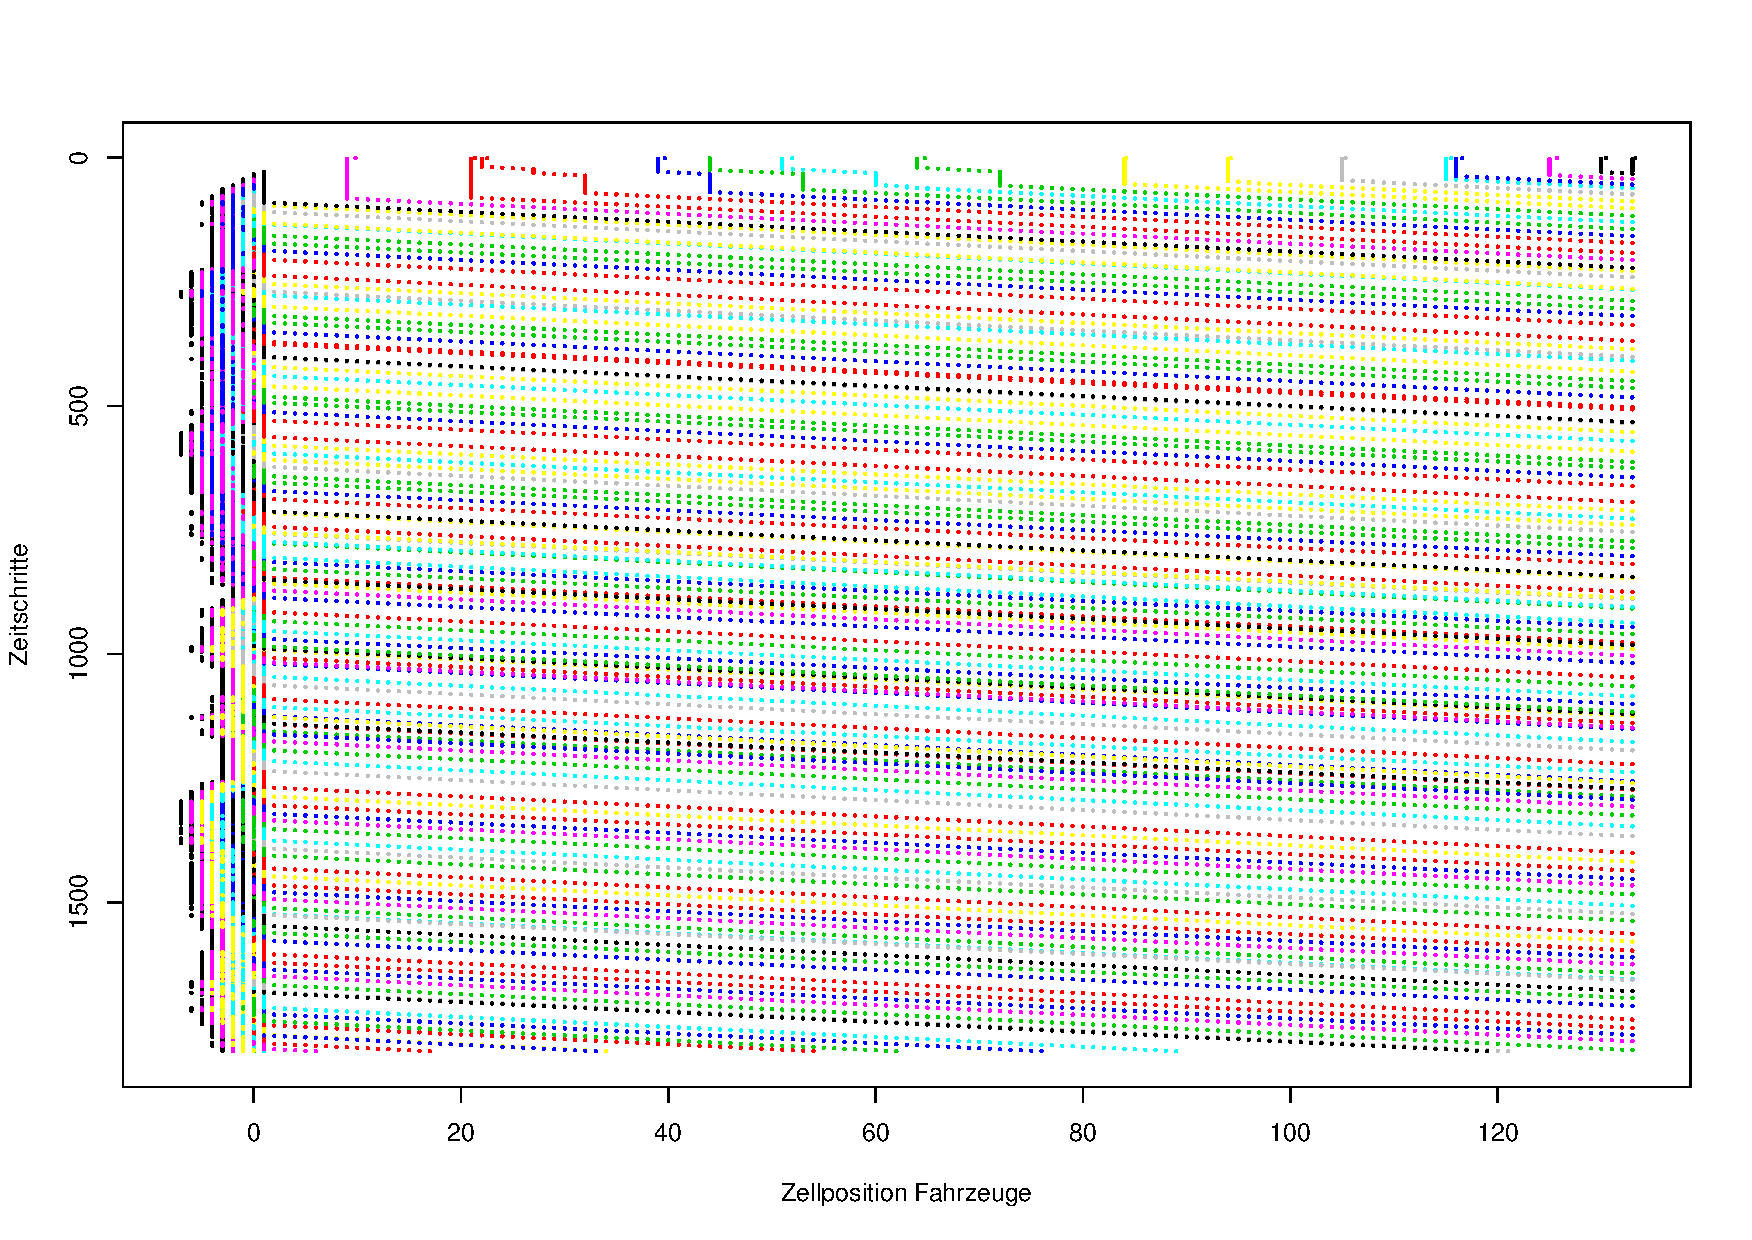
\includegraphics[width=0.9\textwidth]{negativ-sammeln}
 \caption[Punktehäufung im negativen Bereich]
 		{Deutliche Häufung der Punkte im negativen Bereich (Position-Zeit-Diagramm)}
 \label{figure:negativ-sammeln}
\end{figure} 

In \cref{figure:view-range-no-clip} wird die Problematik beispielhaft am Sichtfeld des gelben Fahrzeugs grafisch verdeutlicht. 
Gleiches gilt analog für die rückwärtige Sicht des violetten Fahrzeugs.

\begin{figure}[hptb]
  \centering
    \subfigure[ohne Umbruch]{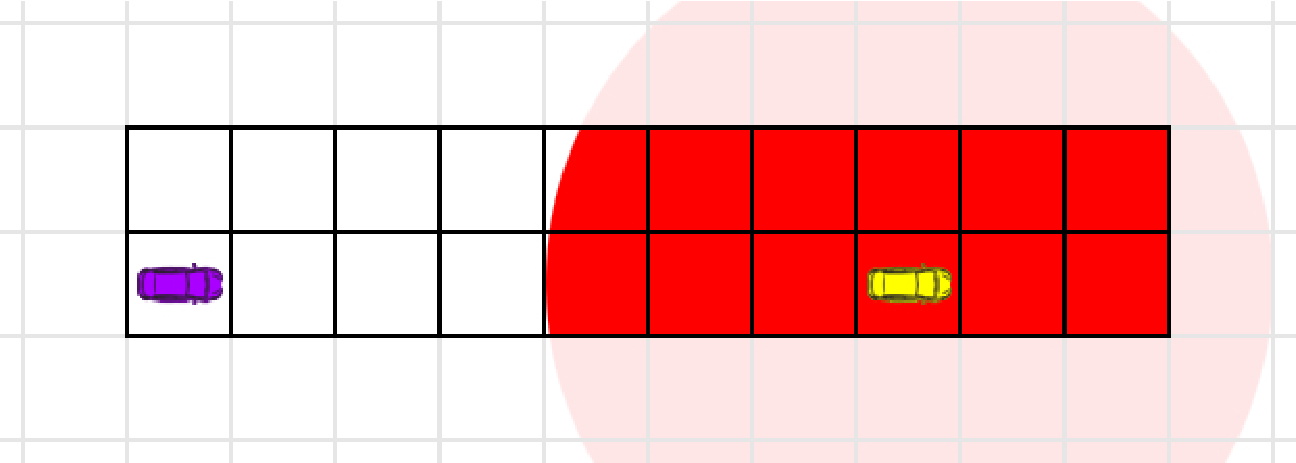
\includegraphics[width=0.8\textwidth]{view-range-no-clip}\label{figure:view-range-no-clip}} \\
    \subfigure[mit Umbruch]{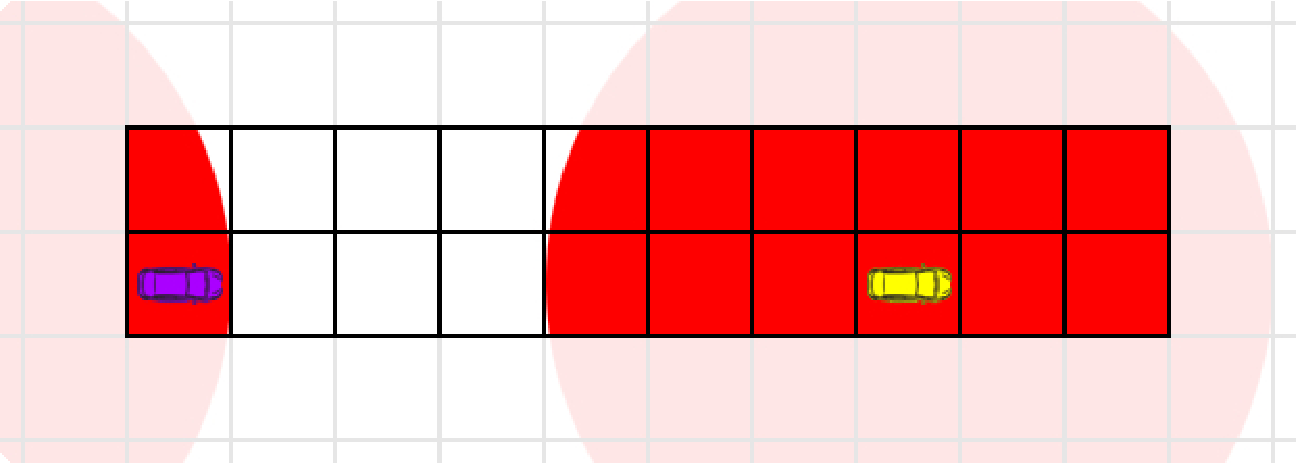
\includegraphics[width=0.8\textwidth]{view-range-clip}\label{figure:view-range-clip}}
  \caption{Sichtfeld des gelben Fahrzeugs, Quelle: Auto-Silhouette vecteezy.com}
  \label{figure:view-range-no-clip-clip}
\end{figure}

Für die Erstellung der sichtbaren Umgebung der Fahrzeuge werden die Zellen zur \enquote{view range}, die sich innerhalb der im Szenario angegebenen Entfernung befinden.
Diese werden als relative Angaben mit dem jeweiligen Fahrzeug als Mittelpunkt gespeichert und in jedem Zeitschritt auf reale Koordinaten umgerechnet.
Befindet sich dann ein anderes Fahrzeug in einer dieser Zellen, befindet es sich im Sichtfeld und eine Entfernung und Richtung wird berechnet.

Die Schwierigkeit bestand darin, die Zellen am anderen Ende der Strecke mit in die Liste der relativen Zellpositionen aufzunehmen, siehe \cref{figure:view-range-clip}.

\sa{own: noch nicht vollends behoben}
Nach der Behebung dieses Fehlers konnten dann auch Stauwellen beobachtet werden, die sich vom Streckenanfang herüber hinaus am Streckenende fortsetzten. 



\subsubsection{Unterteilung des Sichtfeldes der Fahrzeuge}
\label{sec:unterteilung-sichtfeld}

Um die relative Position eines anderen Fahrzeugs in der Umwelt festzustellen, kann die Richtung, in der dieses sich befindet, bestimmt werden.
Die Simulationssoftware hatte für das Sichtfeld der Fahrzeuge eine Unterteilung in acht Sektoren vorgesehen, so dass neben den Richtungen vorwärts, rückwärts, links und rechts auch Unterscheidung in Zwischenschritte links vorwärts, rechts vorwärts usw. möglich war, siehe \cref{figure:car-view-8sectors}.

\begin{figure}[hptb]
  \centering 
   \subfigure[acht Sektoren]{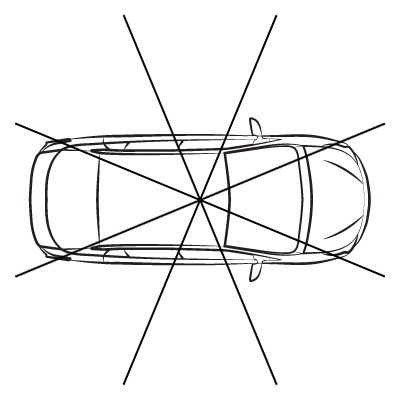
\includegraphics[width=0.3\textwidth]{car-view-8sectors}\label{figure:car-view-8sectors}}\qquad 
   \subfigure[zwei Sektoren]{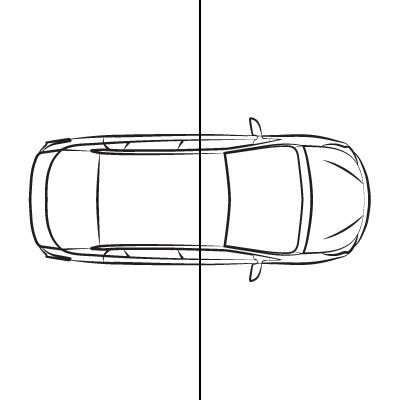
\includegraphics[width=0.3\textwidth]{car-view-2sectors}\label{figure:car-view-2sectors}}\qquad 
   \subfigure[vier Sektoren]{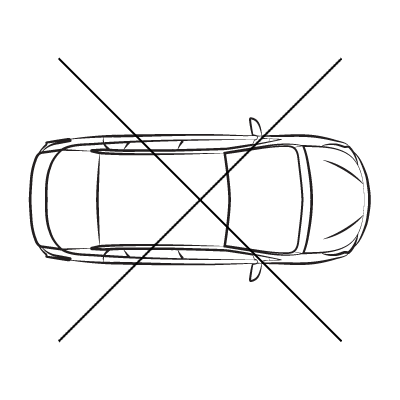
\includegraphics[width=0.3\textwidth]{car-view-4sectors}\label{figure:car-view-4sectors}}
  \caption{mögliche Unterteilung des Sichtfeldes, Quelle: Auto-Silhouette vecteezy.com} 
  \label{figure:car-view-sectors}
\end{figure}

Eine solch feine Unterscheidung war nicht nötig.
Es sollte genügen, feststellen zu können, ob sich ein anderes Fahrzeug relativ zu \enquote{Ego} im vorwärtigen oder rückwärtigen Raum befindet, siehe \cref{figure:car-view-2sectors}. 
Die Abdeckung der Umwelt sollte dabei ohne Unterbrechung sein.
Für die Simulation nach dem Einspurmodell von Nagel-Schreckenberg funktionierte dies ohne Probleme.

Bei einem Testlauf des Mehrspurmodells mit vier Fahrzeugen kam es allerdings zur Kollision zweier Fahrzeuge. 
Bei der Kontrolle des Logs wurde festgestellt, dass ein Fahrzeug (\texttt{vehicle0}), welches sich auf der Überholspur (lane 2) befand, ein anderes Fahrzeug (\texttt{vehicle20}) direkt neben sich nicht \enquote*{gesehen} hatte. 
Erkennbar in der Zeile \enquote{\texttt{PIA1}}, die nur ausgelöst wurde, wenn sich keinerlei Verkehr im Sichtfeld des Fahrzeuges befindet.
Es gab in dieser Konstellation demnach keine Zuordnung dieser Position zu einer der beiden Bereiche.
Daraufhin, so wie es das Verhalten des Agenten vorsah, wurde zum nächsten Schritt (366) in die Hauptspur gewechselt. 
Im diesem Zeitschritt kam es dann zum Auslösen des Kollisionsereignissen, da der Abstand zwischen \texttt{vehicle0} und \texttt{vehicle20} nicht ausreichend groß ist, um das hintere Fahrzeug mit seiner aktuellen Geschwindigkeit zu bewegen.

\footnotesize\begin{verbatim}
--- step 365 ----------------
         vehicle20   in lane   1   in cell   333.0   @   74.21582362319865   kph
         vehicle2   in lane   1   in cell   282.0   @   129.99324819683062   kph
         vehicle0   in lane   2   in cell   333.0   @   99.94723620551235   kph
PIA1     vehicle0   sees no traffic at all -> Pull-in
         vehicle1   in lane   1   in cell   90.0   @   130.8321253026147   kph
--- step 366 ----------------
         vehicle20   in lane   1   in cell   4.0   @   74.21582362319865   kph
         vehicle2   in lane   1   in cell   289.0   @   131.11124225593747   kph
         vehicle0   in lane   1   in cell   3.0   @   100.80986539456516   kph
TFC100   vehicle0   has vehicle in-front of -> decelerate
COS      vehicle0   STOPPED -> collision
OUT      vehicle0   -> Pull-out attempt successful
         vehicle1   in lane   1   in cell   97.0   @   130.64144521630223   kph
\end{verbatim}
\normalsize

Das Sichtfeld der Fahrzeuge wurde zu einem Vier-Sektoren-Modell abgewandelt, siehe \cref{figure:car-view-4sectors}, und die Pläne für Ein- und Ausscheren, der hiervon gleichermaßen betroffen sein dürfte, angepasst.
Es werden nun jeweils die beiden Sektoren kontrolliert, die die Bewegungs- bzw. Orientierungsrichtung darstellen. 
Nach vorn und hinten wird jeweils auch auf Entfernungen geprüft, seitlich auf reine Präsenz/Nichtpräsenz von anderen Fahrzeugen.

Im Rahmen dieser Umstellung wurde festgestellt, dass es bei der Richtungsbestimmung einen Fehler im Framework gab.
Die Berechnung lieferte für beide seitlichen Richtungen ein und denselben Wert.
Der Fehler lag in der Verwendung der Methode \texttt{acos} entstanden, wobei nicht beachtet wurde, dass der arccos nur im Bereich 0 bis $ \pi $ definiert ist, hier aber der Vollkreis zugrunde liegt.





\subsection{Entwicklung des Agentenverhaltens}
\label{sec:entwicklung-agentenplan}

Die mathematischen Gleichungen in \cite{na-sch} beschreiben gut, welches Verhalten dem Agenten zu geben ist: 
\begin{itemize}
	\item wenn möglich beschleunigen
	\item zufällige Reduktion der Geschwindigkeit (Trödeln)
	\item wenn nötig abbremsen
\end{itemize}

\subsubsection{Zustandsautomat}

Dieses Verhalten wurde mit einem endlichen Automaten beschrieben, siehe \cref{figure:fsm-nasch}.

\begin{figure}[hptb]
 \centering
 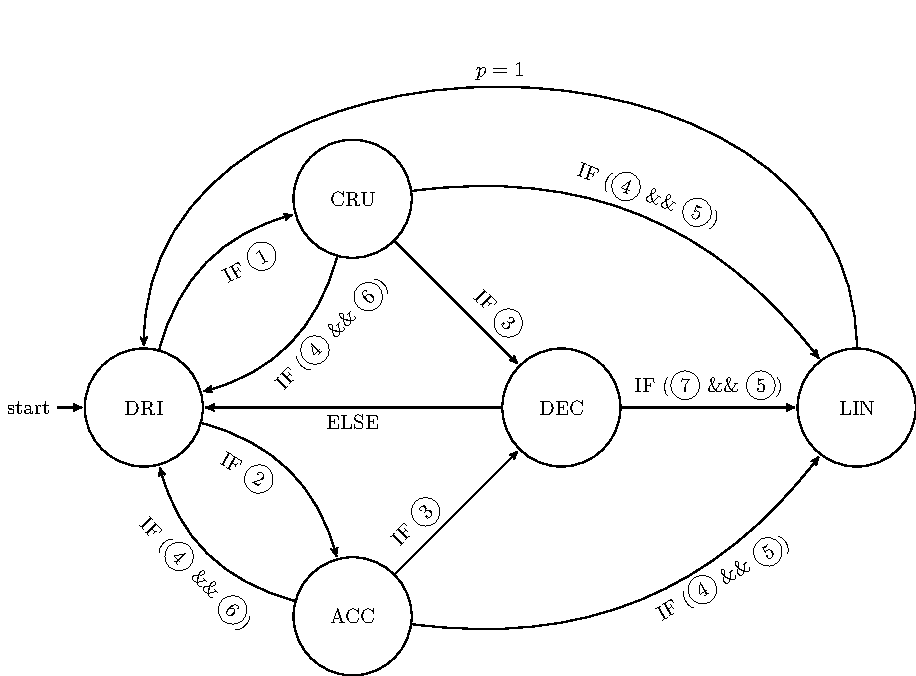
\includegraphics[width=0.9\textwidth]{fsm-nasch}
 \caption[Zustandsautomat für das Agentenverhalten]
 		{Zustandsautomat für das Agentenverhalten nach dem Nagel-Schreckenberg-Modell}
 \label{figure:fsm-nasch}
\end{figure}

Erläuterungen zu \cref{figure:fsm-nasch}:
\begin{enumerate}
\itemsep0em
	\item  $ v_{aktuell}  >=  v_{limit} $
	\item  $ v_{aktuell}  <  v_{limit} $
	\item  \enquote{Verkehr voraus}
	\item  \enquote{kein Verkehr voraus} UND $ p_{linger} $
	\item  \enquote{kein Verkehr voraus} UND $ 1 - p_{linger} $
	\item  $ v_{aktuell}  > 0 $ UND $ p_{linger} $
\end{enumerate}


Startzustand ist ein allgemeiner Zustand \texttt{DRI} (Drive/Fahren), in dem nichts am Verhalten des Agenten geändert wird.
Von hier aus ist der Zustand \texttt{ACC} (Accelerate/Beschleunigen) zu erreichen, wenn die aktuelle Geschwindigkeit unter der max. zulässigen liegt. 
Der Zustand \texttt{CRU} (Cruisen) wird erreicht, wenn die max. zulässige Geschwindigkeit erreicht oder überschritten ist.

Die Übergänge aus den zwei letztgenannten Zuständen sind identisch. 
Ist kein vorausfahrender Verkehr vorhanden und wird nicht getrödelt erfolgt der Übergang zurück in den normalen \texttt{DRI}-Zustand.
Wird stattdessen zufällig mit Wahrscheinlichkeit $ p_{linger} $ das Trödeln angestoßen, wird der entsprechende Zustand \texttt{LIN} erreicht.
Ist Verkehr voraus, wird der Zustand \texttt{DEC} (Decelerate/Verzögern, Bremsen) erreicht.

Aus dem \texttt{DEC}-Zustand kann zufällig ein Übergang in den \texttt{LIN}-Zustand erfolgen ansonsten zurück in den allgemeinen \texttt{DRI}-Zustand.
Aus dem \texttt{LIN}-Zustand wird zwangsläufig wieder in den \texttt{DRI}-Zustand übergegangen.

\subsubsection{Agentenplan}

Der o.g. Automat wurde in die Agentensprache \enquote{übersetzt}. 
Die Automatenversion wurde während der Entwicklung leicht abgeändert. 

Der Agent beginnt im Plan \enquote{\texttt{cruise}}, von dem aus alle weiteren Pläne (\enquote{\texttt{accelerate}}, \enquote{\texttt{linger}}, \enquote{\texttt{decelerate}}) gestartet werden.
Außerdem ruft sich der Plan selbst wieder auf.
\\
Während der Simulationsläufe diente dieser Plan zudem dem Loggen der Statusdaten.
Das komplette Listing siehe \sa{why not} \cref{lst:nasch}.

\begin{lstlisting}[style=asl, 
                   keywords={!cruise}, 
                   keywords={[2]}, 
                   keywords={[3]}, 
                   caption={Auszug aus Agentenscript: Standardplan},
                   label={lst:nasch-auszug}]      
!cruise.

// --- start all other plans ---
+!cruise <-
    !accelerate;
    !decelerate;
    !linger;
    !cruise
.\end{lstlisting}


Der \texttt{accelerate}-Plan war ursprünglich mit der Bedingung ausgestattet, dass die Beschleunigung nur erfolgen soll, wenn die aktuelle Geschwindigkeit unter der zulässigen liegt.
Hier ergab sich das Problem, dass auch bei vorwärtigem Verkehr eine Beschleunigung durchgeführt wurde und die nachfolgende Verzögerung diesen Geschwindigkeitszuwachs in jedem Zeitschritt zusätzlich abbauen musste.
Die Fähigkeit zu verzögern war entsprechend schlecht.

Gelöst wurde dies durch den Zusatz, dass eine Beschleunigung ebenfalls ausbleiben soll, wenn sich ein Fahrzeug im vorwärtigen Sichtbereich befindet.
Mit der Vergrößerung des Sichtfeldes, siehe \cref{sec:sichtweite}, wurde es nötig, außerdem die Entfernung mit in die Bedingung aufzunehmen, ab der nicht mehr beschleunigt werden soll.

Um einen realen Folgeverkehr zu ermöglichen erfolgt die Ausnahme, dass dennoch beschleunigt werden darf, solange das Folgefahrzeug langsamer ist.

Der \texttt{linger}-Plan modelliert das zufällige Verringern der Geschwindigkeit. 
Mit einer Wahrscheinlichkeit von $10 \%$ wird das Trödeln ausgeführt.
Die Intensität der Verzögerung wurde nach einigen Tests, siehe \cref{sec:lingersweetspot}, auf den Wert 0,3, was 30 $\%$ der Bremskraft entspricht, festgelegt.

Die Verzögerung des Agenten wird durch den \texttt{decelerate}-Plan gesteuert. 
Dort wird das Abbremsen bei vorwärtigem Verkehr geregelt. 
Auch hier wurde es nach Erweiterung des Sichtfeldes nötig, zusätzliche Bedingungen für die relative Geschwindigkeit und einen Abstand zwischen den Fahrzeugen einzufügen, um die Lücke nicht zu groß werden zu lassen.

Die realistische Modellierung der Geschwindigkeitsänderungen macht es unmöglich, dass sich die Fahrzeuge in aufeinanderfolgenden Zellen folgen.
Vielmehr muss, wie im realen Verkehr auch, ein gewisser Abstand, innerhalb dessen der Nachfolgeverkehr reagieren kann, eingehalten werden.
Ein Wert von 100 m erschien in der Simulation sinnvoll, um Kollisionen zu verringern. 
Für eine Geschwindigkeit von 100 km/h entspricht diese Entfernung nach der Faustformel, siehe \cite{bremsweg}, dem Bremsweg.

Ist der Geschwindigkeitsunterschied zwischen Fahrzeugen allerdings zu groß, können diese nicht verhindert werden.


\paragraph{Tests des Agentenplanes}

Um die Wirksamkeit der Anweisungen für die Agenten zu testen, wurden in der Szenariovereinbarung zwei Arten von Fahrzeugen, welche mit identische Plänen ausgestattet waren, zum Einsatz gebracht.
Der einzige Unterschied, den es zwischen den Fahrzeugen gab, war, dass eines seine Geschwindigkeit aus einem niedrigeren Intervall wählen musste.
\\
Somit war sichergestellt, dass das schnellere Fahrzeug im Laufe der Simulationzeit auf das langsamere aufholen würde.
Es war wiederholbar zu testen, ob das Abbremsen bei vorwärtigem Verkehr funktionierte.

%\begin{figure}[hptb]
%  \centering 
%   \subfigure[Zellpostionen]{\includegraphics[width=0.5\textwidth]{image1name}\label{figure:image1name}}\qquad 
%   \subfigure[Geschwindigkeit]{\includegraphics[width=0.5\textwidth]{image2name}\label{figure:image2name}}
%  \caption{lalala} 
%  \label{figure:imagename}
%\end{figure}























%%.\sa{hier vermischst Du \cref{sec:sota} mit \cref{sec:realisierung}, hier geht es darum, wi Du konkret arbeiten willst um die Sachen unter \cref{sec:researchgap} zu beweisen oder zu belegen, evtl macht es Sinn diese Punkte mit in \cref{sec:sota} zu ziehen, Du kannst dann einfach, wenn Du es brauchst Verweise setzen}
%
%\noindent
%Die in \cite{dat-ba} vorgeschlagene Struktur ist zu implementieren und in vergleichbarer Umgebung simulatorisch zu testen. 
%Dabei sind die folgenden Größen zu erheben und entsprechend statistisch auszuwerten: 
%
%\begin{itemize}
%\item Verkehrsdichte
%\item Verkehrsfluss
%\item Spurwechselfrequenz
%\item Spurnutzung links/rechts
%\end{itemize}
%
%Das Testszenario wurde in \cite{na-sch} durch das zu Beginn zufällige Platzieren von Fahrzeugen in einem geschlossenen Kreis mit $L$ Zellen (ähnlich einer Autorennstrecke) simuliert. \\
%Allerdings wurde auch, bei der Simulation einer Fahrbahnverengung, eine Alternative Simulationsmöglichkeit beschrieben. 
%Eine Gridgerade von bis zu 10000 Zellen Länge wurde getestet - Bewegungsrichtung von links nach rechts. 
%Die Fahrzeuge wurden mit $v=0$ in die am weitesten links befindliche Zelle, so diese frei war, gesetzt und die Fahrzeuge in den sechs am weitesten rechts befindlichen Zellen (bei systemweiter $v_{max}=5$) gelöscht. 
%Letzteres Vorgehen sorgte für eine offene Grenze für den abfließenden Verkehr.
%
%Für eine kontinuierliche Simulation ist die zweite Möglichkeit ungeeignet. 
%Auch in \cite{multi-lane} wird von der Nutzung periodischer Randbedingungen gesprochen. 
%Dies lässt darauf schließen, dass, wie in \cite[Abb. 1.5]{peri-rand} für die Umgebung von Pixeln beschrieben, die Fahrzeuge vom \enquote*{Ende} der Gridstrecke am \enquote*{Anfang} wieder eingesetzt wurden und somit der zuerst beschriebene Kreis einsteht.
%Dieses Verhalten ist zu bevorzugen.
%
%Vorteil der geschlossenen Kreisstrecke ist, dass man bei konstanter Fahrzeuganzahl $N$ (bei \cite{multi-lane} waren dies $N = 10^{3}$) durch die Veränderung der Systemgröße eine unterschiedliche Fahrzeugdichte erreicht werden kann. 
%Jeder Dichtewert wurde für $T = 10^{5}$ Zeitschritte simuliert, wobei die erste Hälfte verworfen wurde, um mögliche Störeffekte ausklingen zu lassen. 
%Die generierten Simulationsdaten wurden über $T_{sample} = 300$ Zeitschritte und eine Wegstrecke von 133 Zellen, was etwa 1 km Länge in der realen Welt entspricht, gemittelt, um statistische Schwankungen zu reduzieren.
%
%Ein mögliches Simulationstool ist das \enquote{Traffic Simulation Game}\footnote{\link{https://lightjason.github.io/news/2017-09-workshop/}}. 
%In der Grundkonfiguration erzeugt dieses eine beliebig lange, gerade Straße mit beliebig vielen Fahrspuren. 
%ſEs ist zu prüfen, ob die Software auf die gewünschte Verhaltensweise angepasst werden kann.